% Latex Beamer template following CERN template guidelines (or trying!)

\documentclass[aspectratio=169]{beamer}
\usepackage{xcolor}
\usepackage{graphicx}
\usepackage{multicol}
\usepackage{tikz}

% Code listings with syntax highlighting
%  Require Pygments
\usepackage{minted}

\usetheme{CERN}


% Talk date
% Uncomment this to define a presentation date distinct from \today
\def\mydate{11 Oct 2018}

% Preamble
\title[]{Readout System Enhancements for ATLAS ITk Project }
\subtitle{}
\author[Kyle Beyer , Dylan Hatch]{Kyle Beyer, \texorpdfstring{\url{kyle.beyer@cern.ch} \\ Dylan Hatch,  \url{dylan.brown.hatch@cern.ch}}{Kyle Beyer , Dylan Hatch}}

% Body
\begin{document}

    \cernSplashBlue

    % Title
    {
    \setbeamertemplate{footline}{}
    \setbeamertemplate{navigation symbols}{}
    \frame{\titlepage

      \begin{tikzpicture}[remember picture, overlay]
        \node[anchor=south west, %anchor is bottom left corner of the graphic
              xshift=0.5cm, %shifting around
              yshift=0.5cm]
       at (current page.south west) %left bottom corner of the page
        { \includegraphics[width=0.3\paperwidth]{images/mlogo.png} };

        \node[anchor=south east, %anchor is bottom left corner of the graphic
              xshift=-0.5cm, %shifting around
              yshift=0.3cm]
       at (current page.south east) %left bottom corner of the page
        {	\includegraphics[width=0.23\paperwidth]{images/wlogo.png} };
			\end{tikzpicture}

    }

    \setcounter{framenumber}{0}

    % TOC
%     \frame{
%        \frametitle{Agenda}
%        \begin{multicols}{2}
%            \tableofcontents
%        \end{multicols}
%    }

%%%%%%%%%%%%% Begin Dylan Stuff %%%%%%%%%%%%%%%%%%%%%%%%%%%%%%%%%%%%%%%%%%%%%%%%

    \frame{
        \frametitle{Current DAQ Readout Chain}
        \begin{columns}[c]
            \column{0.75\textwidth}
            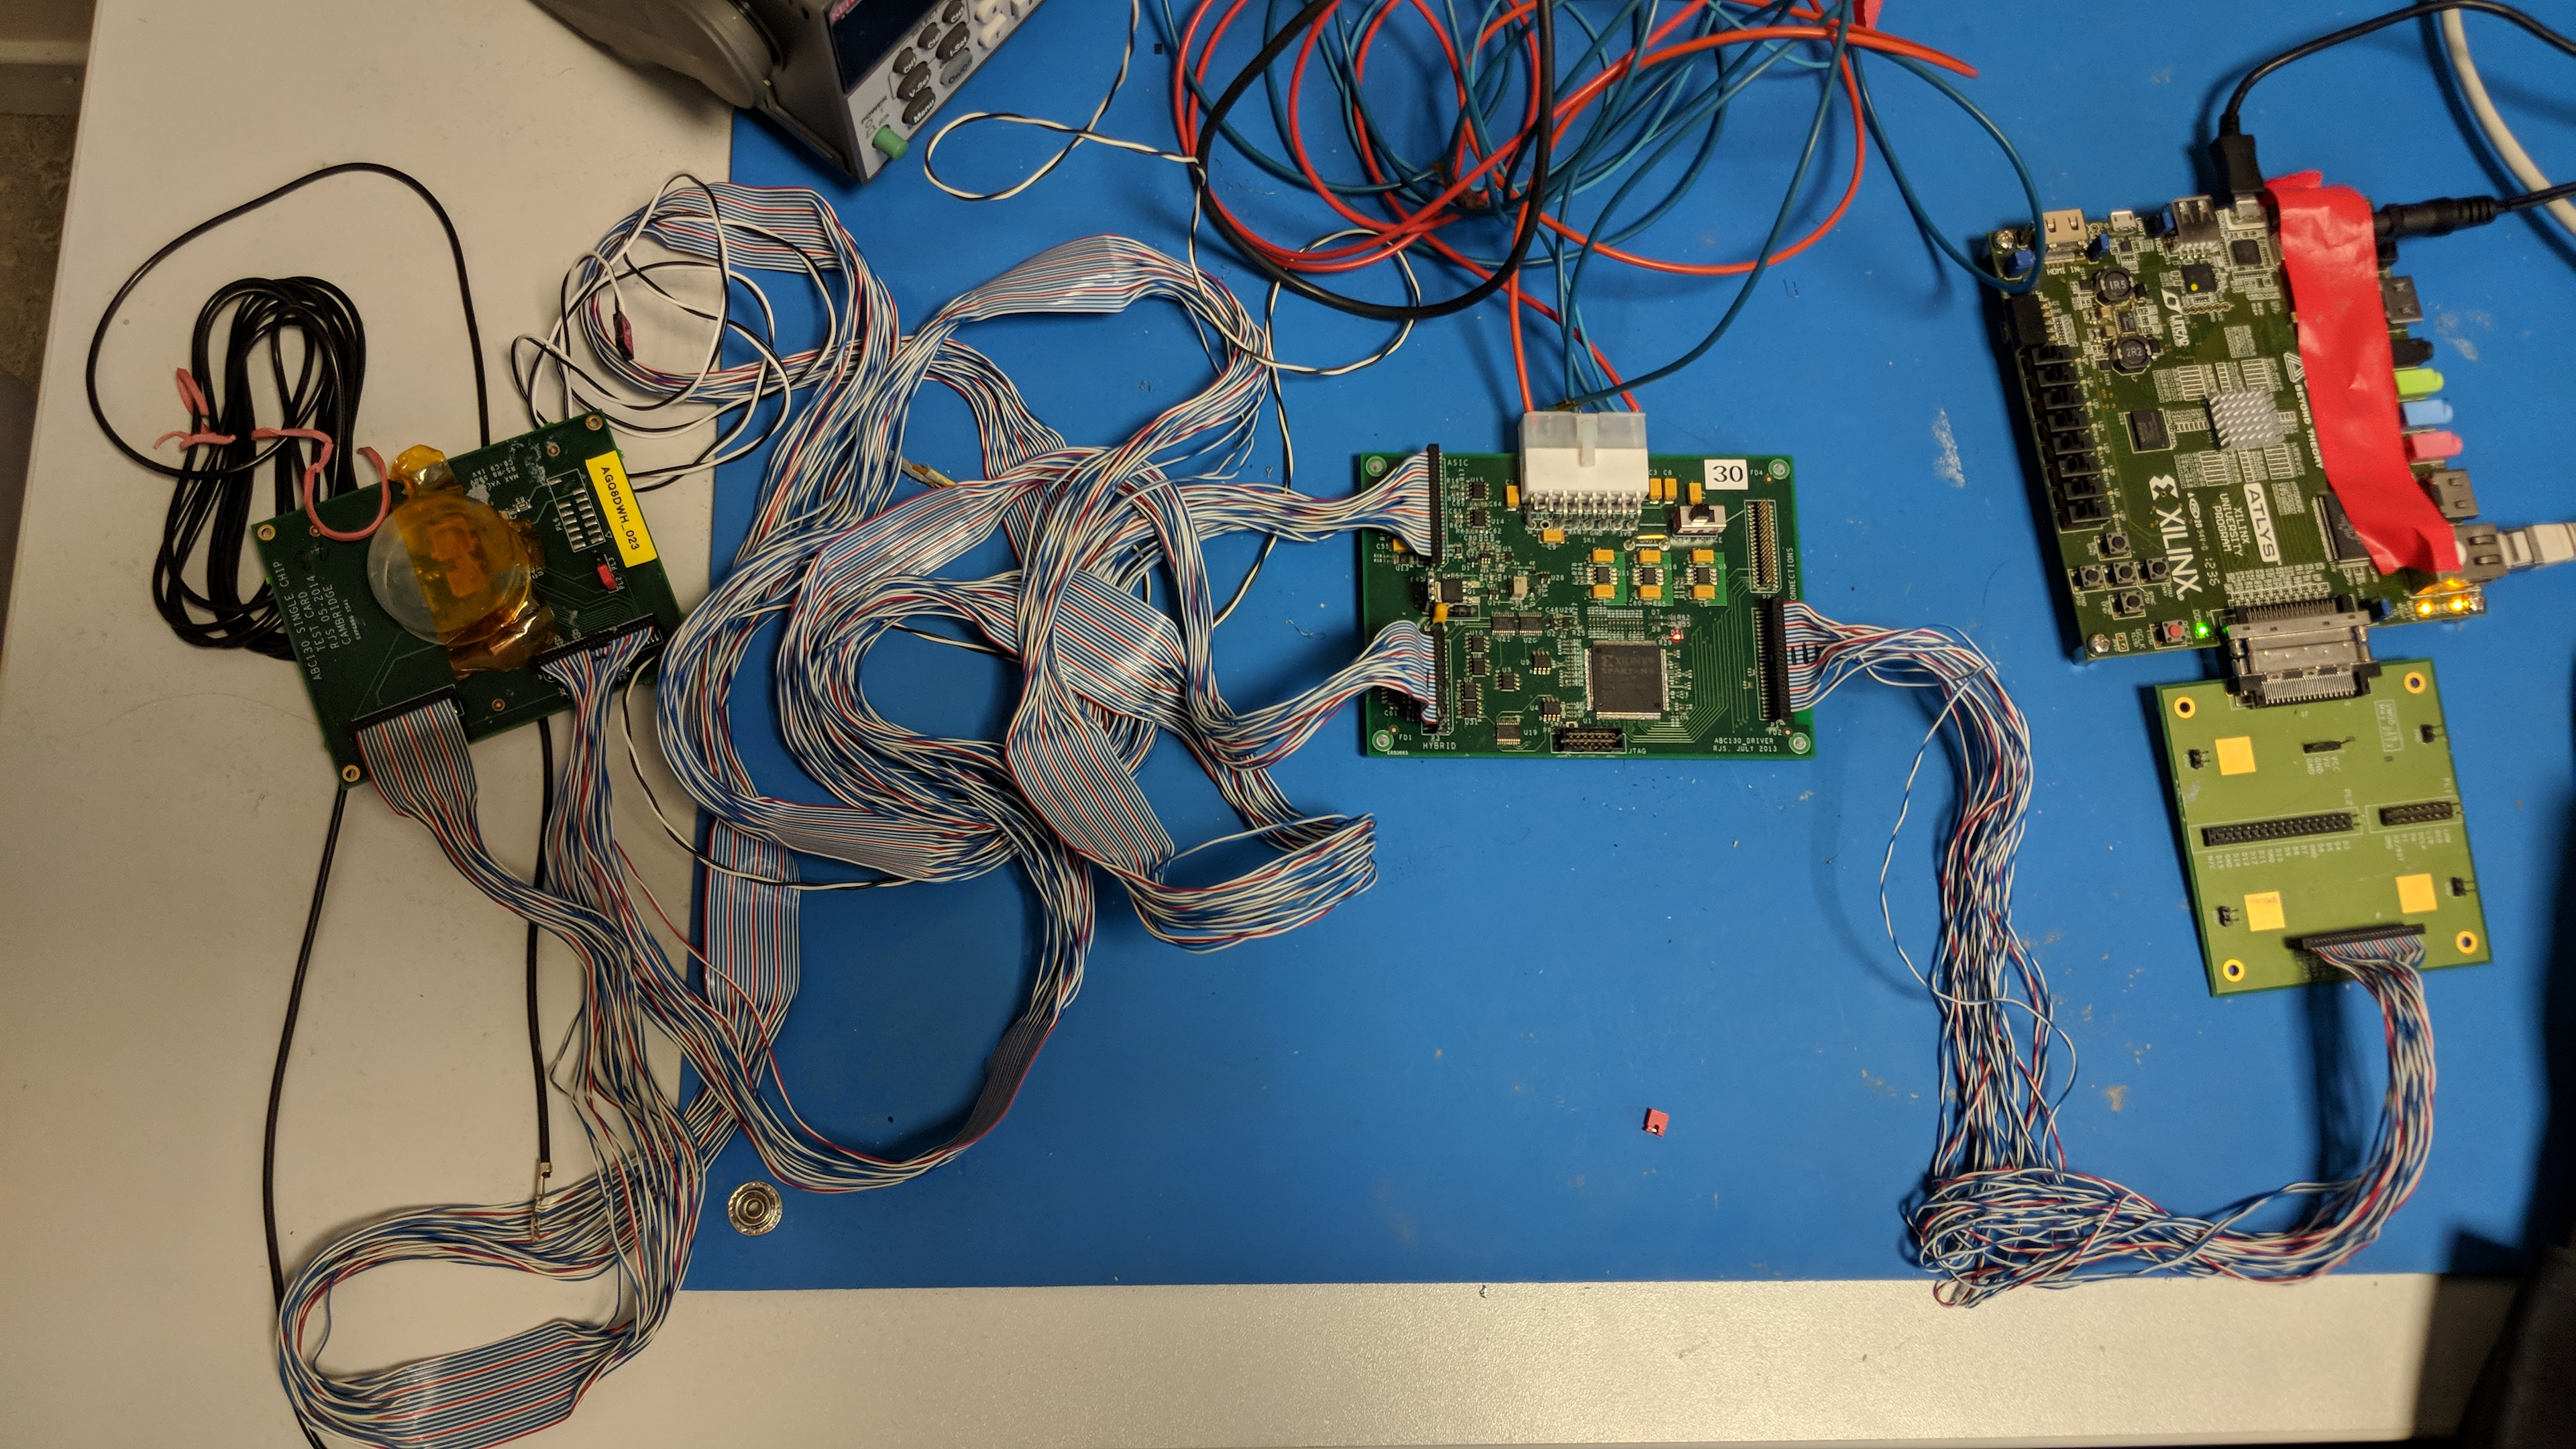
\includegraphics[width=1.0\textwidth]{images/readout_chain.jpg}

            \column{0.25\textwidth}
            A look at the fully assembled readout chain.
        \end{columns}
    }

    \frame{
        \frametitle{ATLYS Board}
        \begin{columns}[c]
            \column{0.5\textwidth}
            \includegraphics[width=1.0\textwidth]{images/atlys_pic.png}

            \column{0.5\textwidth}
            ATLYS is a low cost, widely available board that supports single chip, hybrid, and module tests.
        \end{columns}
    }

    \frame{
        \frametitle{Interface Connection}
        \begin{columns}[c]
            \column{0.7\textwidth}
            \includegraphics[width=1.0\textwidth]{images/ATLYSwithVMOD-IB.jpg}

            \column{0.3\textwidth}
            The ATLYS board is connected to to its interface board, VMOD-IB.
        \end{columns}
    }

    \frame{
        \frametitle{Hybrid Board}
        \begin{columns}[c]
            \column{0.7\textwidth}
            \includegraphics[width=1.0\textwidth]{images/hybrid_board.jpg}

            \column{0.3\textwidth}
            Orientation of the power, ABC130, and ATLYS connections.
        \end{columns}
    }

    \frame{
        \frametitle{ABC130 Single Chip Test Card}
        \begin{columns}[c]
            \column{0.4\textwidth}
            \includegraphics[width=1.0\textwidth]{images/ABC130_card.jpg}

            \column{0.6\textwidth}
            Test card, with connection to the Hybrid chip.
        \end{columns}
    }

    \frame{
        \frametitle{Obstacles}
        \begin{itemize}
            \item We accidentally lost a configuration and register assignment file on a formatted Windows SSD.
            \item We have a segmentation violation in the GUI of the ITSDAQ software.
            \item We have a compile error due to the absence of a header file supposedly in the NI-VISA library.
            \item Our new installation of the NI-VISA library has caused problems with gnome on the workstation.
        \end{itemize}
    }


    \frame{
        \frametitle{Acknowledgements}
        We would like to acknowledge the University of Michigan Department of Physics, specifically Jean Krisch and Tom Schwarz, and Steven Goldfarb.

        We would also like to acknowledge the support of the Lounsbery foundation.   \\
        %More content goes here
      \begin{tikzpicture}[remember picture, overlay]
        \node[anchor=south west, %anchor is bottom left corner of the graphic
              xshift=2.4cm, %shifting around
              yshift=0.4cm]
       at (current page.south west) %left bottom corner of the page
        { \includegraphics[scale=0.05,trim={0 0 0 35cm },clip]
        {p1-figs/cham.jpg} };

        \node[anchor=south east, %anchor is bottom left corner of the graphic
              xshift=-2.4cm, %shifting around
              yshift=0.4cm]
       at (current page.south east) %left bottom corner of the page
        {	\includegraphics[width=0.33\paperwidth]{p1-figs/okto.jpg} };
			\end{tikzpicture}


    }

    \section{}
    \cernSplashWhite

\end{document}
